
    \section{引言}

    \subsection{概述}
    \begin{frame}
      \frametitle{概述}
      \begin{itemize}
        \item 图像去雾是一类非常有意义的图像处理问题,它的目标是恢复被雾气遮挡的图像;
        \item 图像去雾的应用场景有很多,比如:交通监控、自动驾驶、遥感观测等;
        \item 图像去雾的算法有很多,这里只介绍基于图像增强、基于物理模型、基于深度学习的三种方法。
      \end{itemize}
    \end{frame}

    \begin{frame}
      \frametitle{概述}
      \begin{figure}
        \centering
        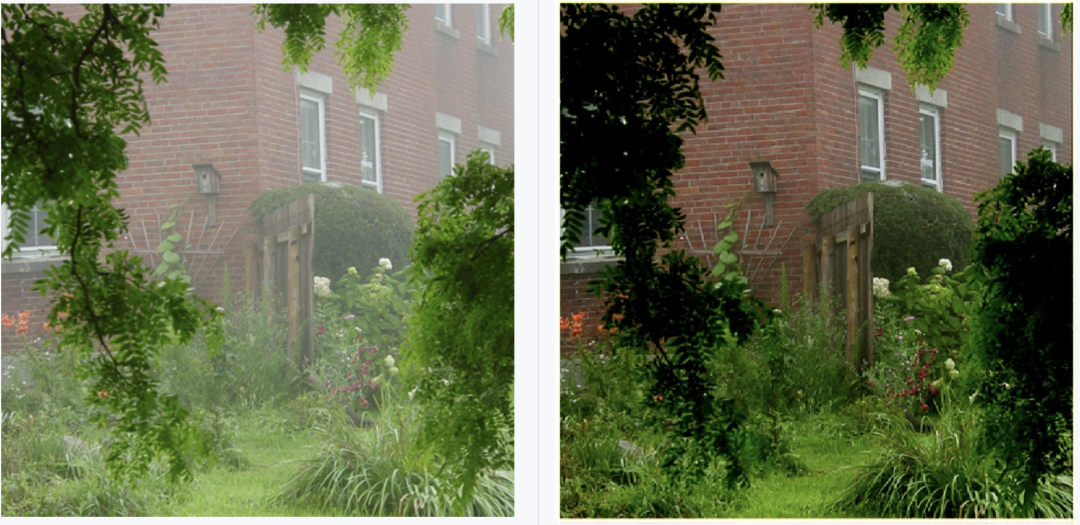
\includegraphics[width=\textwidth]{figures/pic1.png}
        \caption{图像去雾实例}
      \end{figure}
    \end{frame}

    \subsection{算法难点}
    \begin{frame}
      \frametitle{算法难点}
      \begin{itemize}
        \item \textbf{雾图特征有限}: 有雾图像由于受到雾气成像环境的干扰,其亮度、纹理、轮廓、形状等特征都存在不同程度的损失。
        \item \textbf{实时处理问题}: 如果雾图增强或复原花费的计算或存储开销过大,势必极大影响应用系统的实时工作。
        \item \textbf{普适性问题}: 算法面临的最大问题是对不同类型的雾图难以获得一致的增强或复原质量。
      \end{itemize}
    \end{frame}



